\begin{frame}
\frametitle{Ensemble learning}
Combining predictions from weak learners.
\begin{itemize}
\item {\bf Bootstrap aggregating (bagging)}
\begin{itemize}
\item Train several weak classifiers, with different models or randomly drawn subsets of the data.
\item Average their predictions with equal weight.
\end{itemize}
\item {\bf Boosting}
\begin{itemize}
\item A family of approaches, where models are weighted according to their accuracy.
\item AdaBoost is popular, but has problems with target noise.
\end{itemize}
\item {\bf Bayesian model averaging}
\begin{itemize}
\item Really a model selection method.
\item Relatively ineffective for combining models.
\end{itemize}
\item {\bf Bayesian model combination}
\begin{itemize}
\item Shows promise.
\end{itemize}
\end{itemize}
\begin{tiny}
Monteith, et al. ``Turning Bayesian model averaging into Bayesian model combination.'' Neural Networks (IJCNN), The 2011 International Joint Conference on. IEEE, 2011.\par
\end{tiny}
\end{frame}

%\begin{frame}
%\frametitle{Random Forests}
%\end{frame}

\begin{frame}
\frametitle{Boosting}

Reduce sequentially the bias of the combined
estimator. \\

Examples: AdaBoost, Gradient Tree Boosting, ...\\

\begin{center}
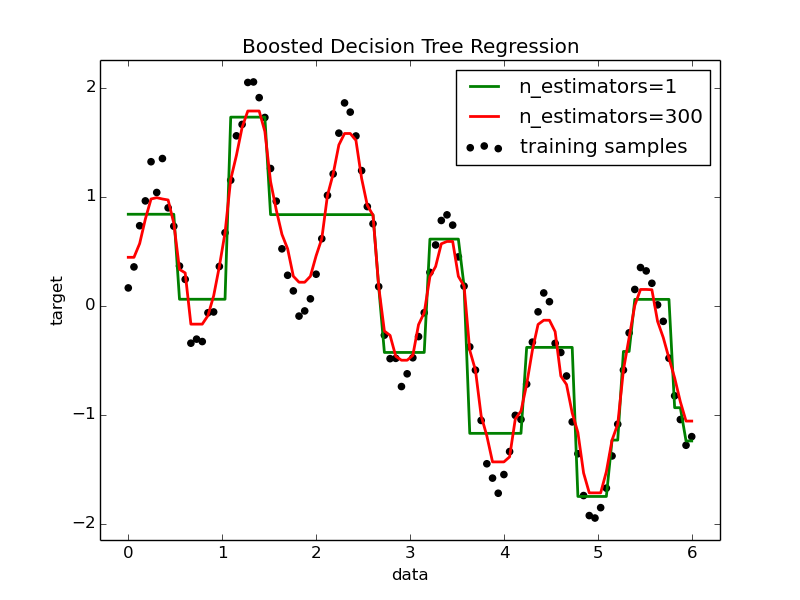
\includegraphics[width=.75\linewidth]{sklearn_material/plot_adaboost_regression.png}
\end{center}

\end{frame}


\begin{frame}
\frametitle{Bagging}

Build several estimators independently and average their
predictions. Reduce the variance.\\

Examples: Bagging methods, Forests of randomized trees, ...\\

\begin{center}
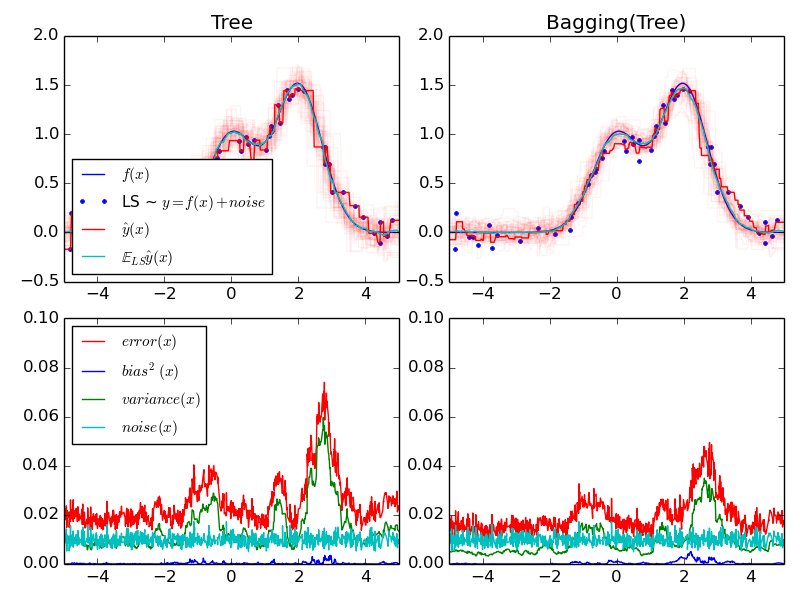
\includegraphics[width=.7\linewidth]{sklearn_material/bias_variance.png}
\end{center}

\end{frame}



\begin{comment}
\begin{frame}
\frametitle{Ensemble learning}
ensemble methods: combine the predictions of several
base estimators (generalizability / robustness)  

\begin{itemize}
\item 
\textbf{averaging methods:} build several
estimators independently and average their predictions. Recuce the variance:\\

Examples: Bagging methods, Forests of randomized trees, ...
\item
\textnf{boosting methods:} reduce sequentially the bias of the combined
estimator. \\

Examples: AdaBoost, Gradient Tree Boosting, ...
\end{itemize}
\end{frame}
\end{comment}


